\documentclass{exam}

\usepackage{units} 
\usepackage{xfrac} 
\usepackage[fleqn]{amsmath}
\usepackage{cancel}
\usepackage{float}
\usepackage{mdwlist}
\usepackage{booktabs}
\usepackage{cancel}
\usepackage{polynom}
\usepackage{caption}
\usepackage{fullpage}
\usepackage{comment}
\usepackage{enumerate}
\usepackage{graphicx}

\newcommand{\degree}{\ensuremath{^\circ}} 
\everymath{\displaystyle}

\printanswers

\ifprintanswers 
  \usepackage{2in1, lscape} 
\fi
\title{Statistics \\ Homework One}
\author{}
\date{January 22, 2014}

\begin{document}

  \maketitle

  \section{Homework}
  \ifprintanswers
  \else
    \begin{itemize*}
      \item read Chapter 1 
      \item answer the questions in ``Check Your Skills.''  Check your answers
        in the back of the book, but you don't have to hand this in.
      \item do exercises: 23-26, 29-35, 37, 39-41, 44-45 (hand in next week)
    \end{itemize*}
  \fi

  \ifprintanswers
    \begin{description}
      \item[23]
        \begin{parts}
          \part Laurie Abrams, Gordon Brown, Maria Cabrera and Miranda Ismael 

          \part
          \begin{tabular}[H]{ll}
            \toprule
            Variable         & Type \\
            \midrule
            Medical School   & categorical \\
            Sex              & categorical \\
            Age              & quantitative \\
            USMILE           & quantitative \\
            Specialty sought & categorical \\
            \bottomrule
          \end{tabular}
        \end{parts}

      \item[24]
        \begin{parts}
          \part categorical
          \part categorical
          \part quantitative
          \part categorical
          \part quantitative
        \end{parts}

      \item[25]
          \[
            other = 100 - 19 - 18 - 16 - 13 - 12 - 12 - 5 = 5
          \]

          \begin{figure}[H]
            \centering
            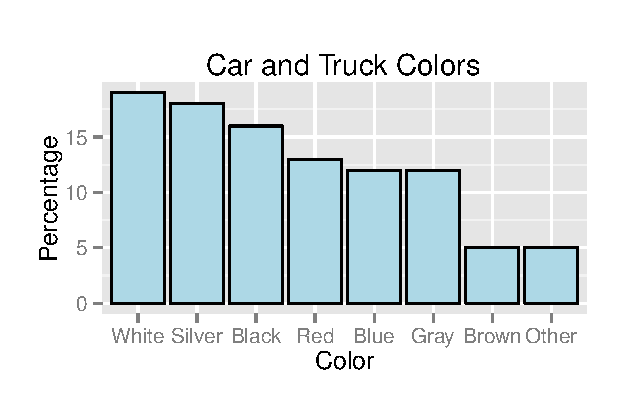
\includegraphics{figures/ex25.eps}
            \caption{Exercise 25}
          \end{figure}

      \item[26]
        The data show the percentage of each age group that bought music.  A
        pie chart might show what percentage of the total online music market
        went to each age group, which is a completely different set of numbers.

        \begin{figure}[H]
          \centering
          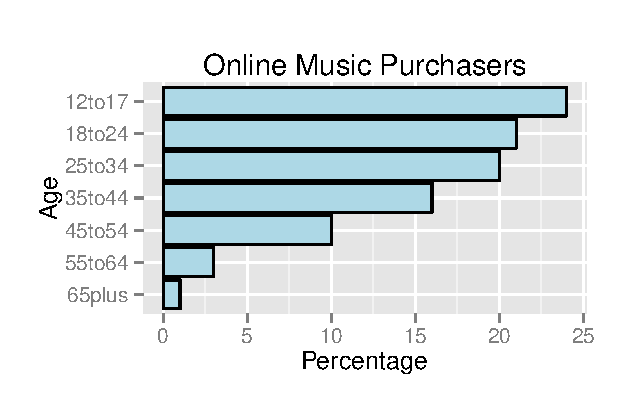
\includegraphics{figures/ex26.eps}
          \caption{Exercise 26}
        \end{figure}

      \pagebreak

      \item[29]
        \begin{figure}[H]
          \centering
          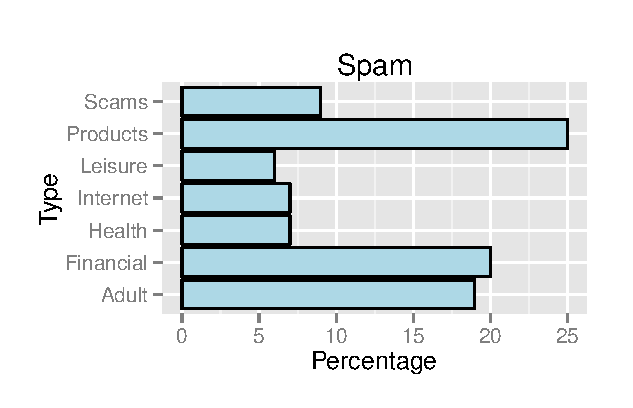
\includegraphics{figures/ex29a.eps}
          \caption{Exercise 29 Ordered Alphabetically}
        \end{figure}

        \begin{figure}[H]
          \centering
          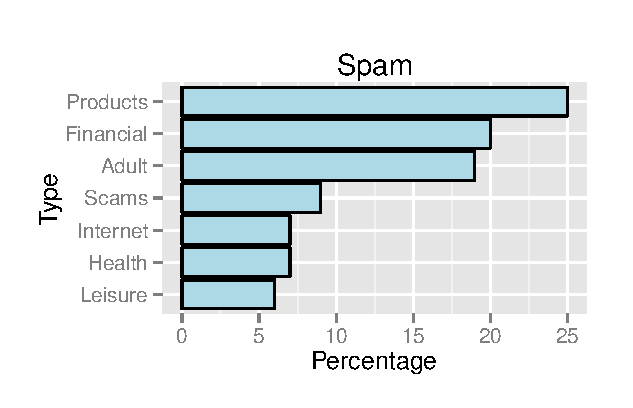
\includegraphics{figures/ex29b.eps}
          \caption{Exercise 29 Ordered by Percentage}
        \end{figure}

      \item[30]
      \pagebreak
        \begin{parts}
          \part
            \begin{itemize*}
              \item The center is around 2 servings--about half the girls eat 2
                or fewer servings and about half the girls eat more than two
                servings.

              \item The data is right-skewed.  
            
              \item The spread is from 0 servings to 8 servings.
            \end{itemize*}

          \part 26 out of 74 or 30\% eat less than 2 servings per day
        \end{parts}

      \item[31]
        \begin{parts}
          \part The shape is symmetric with a center around 110.  Ignoring the
          outliers, the spread is 50 (86 to 136).

          \part 64 out of 78 or 82\% of the students had scores over 100.
        \end{parts}

      \item[32]
        \begin{parts}
          \part Ignoring the outliers, the shape looks symmetric.

          \part The center seems to be around 2\%.

          \part The smallest return was around -12\% and the largest return was around 14\%.

          \part About a third of the months had a return less than zero.
        \end{parts}

      \item[33]
        \begin{enumerate}
          \item Graph b and graph c both have two choices.  The number of
            females/males is probably more even than the number of left
            handed/right handed, so graph c is the female/male graph.

          \item graph b

          \item Graph d is evenly distributed around some average number, so
            this is probably the height.

          \item Graph a shows a bunch of people who don't study at all, with
            gradually diminishing numbers of people who study more hours per
            night.
        \end{enumerate}

      \item[34]
        \begin{parts}
          \part
            \begin{figure}[H]
              \centering
              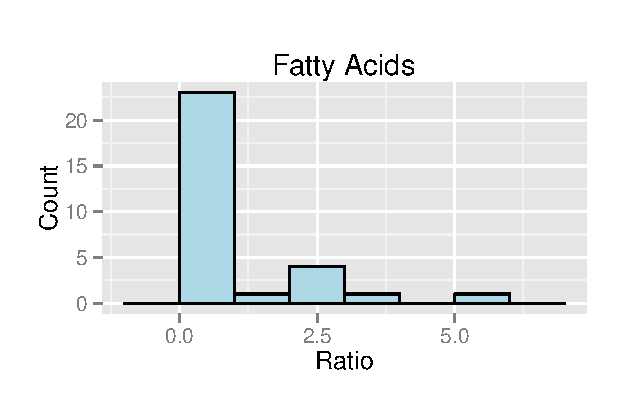
\includegraphics{figures/ex34.eps}
              \caption{Exercise 34}
            \end{figure}

          \part The distribution is left-skewed.  Most of the oils have a low ratio.

          \part All the fish oils have ratios greater than or equal to 2 which
          makes them pretty healthy.

        \end{parts}

      \pagebreak

      \item[35]
        \begin{parts}
          \part Since the states have varying numbers of people, it's more
          interesting to know the ratio of doctors to people than the total
          number of doctors.

          \part 
            \begin{figure}[H]
              \centering
              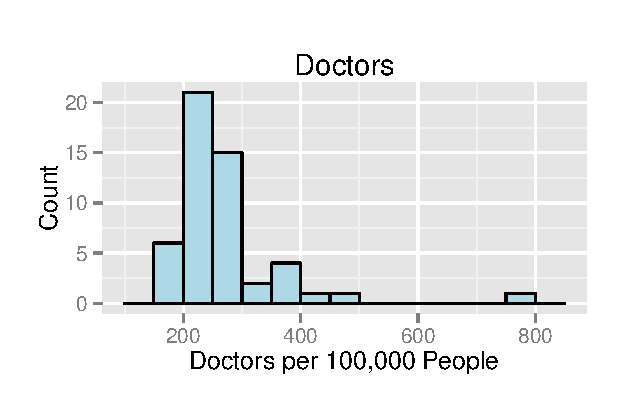
\includegraphics{figures/ex35.eps}
              \caption{Exercise 35}
            \end{figure}

            The histogram is right-skewed with a center around 230.  Washington
            DC is an outlier, probably because it is a city and not a state.

        \end{parts}

      \item[37]
        \begin{figure}[H]
          \centering
          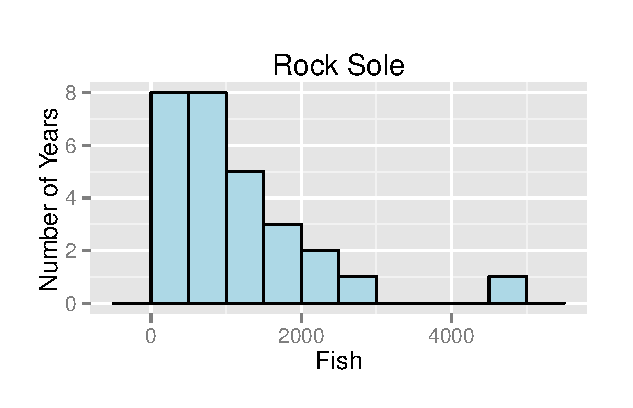
\includegraphics{figures/ex37.eps}
          \caption{Exercise 37}
        \end{figure}

        The histogram is left-skewed with a center around 1000. and a spread of
        3000, ignoring the one outlier.  1987 was an outlier. 

      \item[39]
        \begin{figure}[H]
          \centering
          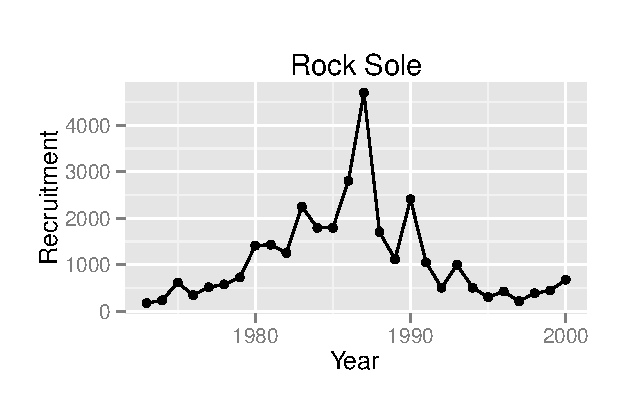
\includegraphics{figures/ex39.eps}
          \caption{Exercise 39}
        \end{figure}

        The fish recruitment increased until 1989 and then declined.

      \item[40]
        \begin{parts}
          \part You would expect the categories with the most drivers to have
          the most accidents, regardless of any effect pot might have.  

          \part 
            \begin{figure}[H]
              \centering
              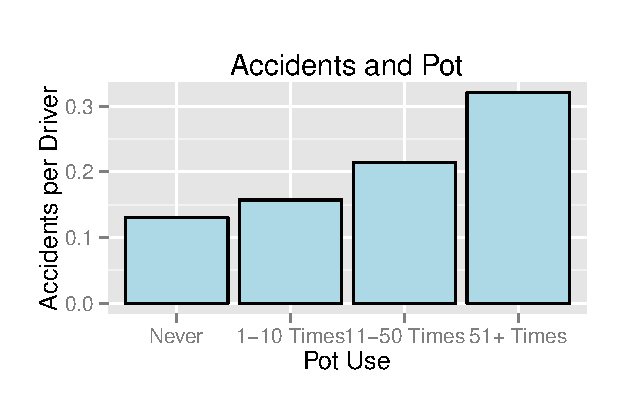
\includegraphics{figures/ex40.eps}
              \caption{Exercise 40}
            \end{figure}

            It looks like the pot smokers tend to get in more car accidents.

        \end{parts}

      \item[41]
        Most coins you would find would probably have been made in the last
        decade.  However, coins have a long life, so you might find a few coins
        which are 40 or 50 years old.

      \item[44]
        \begin{parts}
          \part In each year, the prices are highest around July and lowest around January.  
          
            \part There is a long term year over year increase in the prices.

            \part Prices plummeted in 2007

        \end{parts}

      \item[45]
        \begin{parts}
          \part
            The center is around 13.  About half the years had less than 13
            attacks and about half the years had 13 or more attacks.  

            \begin{figure}[H]
              \centering
              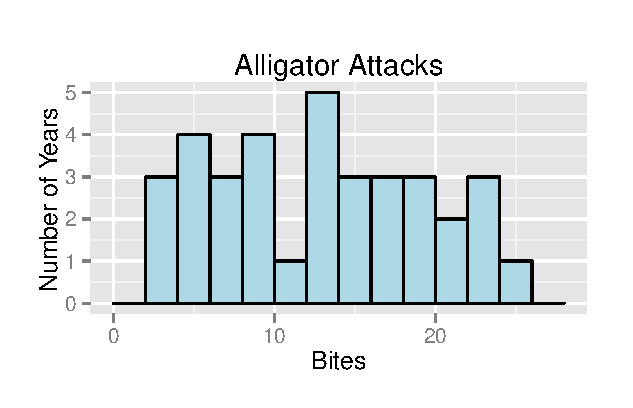
\includegraphics{figures/ex45a.eps}
              \caption{Exercise 45a}
            \end{figure}

          \part
            \begin{figure}[H]
              \centering
              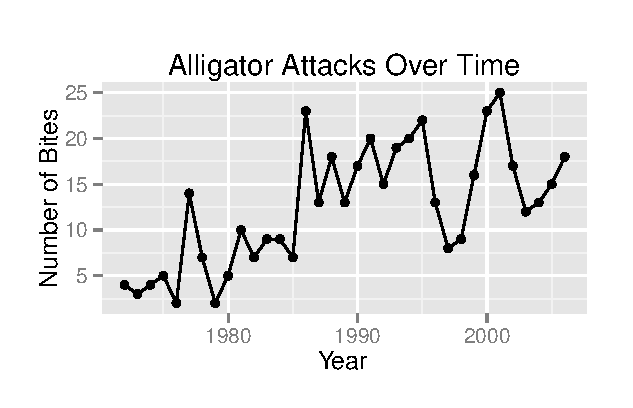
\includegraphics{figures/ex45b.eps}
              \caption{Exercise 45b}
            \end{figure}

            14 of the 21 years between 1986 and 2007 had more than 13 attacks per year.

        \end{parts}


    \end{description}

  \else
    \vspace{10 cm}
    \begin{quote}
      \begin{em}
        The government has failed us; you can't deny that. Anytime you live in
        the twentieth century, 1964, and you're walking around here singing
        ``We Shall Overcome,'' the government has failed us. This is part of
        what's wrong with you---you do too much singing.  Today it's time to
        stop singing and start swinging. 
        
        % You can't sing up on freedom,
        % but you can swing up on some freedom.
        % Power in defense of freedom is greater than power in behalf of tyranny and oppression.
      \end{em}
    \end{quote}
    \hspace{1 cm} --Malcolm X
  \fi

\end{document}

